% Status info:
% A. Wolf	2017
% 20171029 AW: A first version of text
% 20171210 GZ: small changes for finalization.

\chapter{Planetary nomenclature}
\label{ch:Nomenclature}

Planetary nomenclature\newFeature{0.17.0}, like terrestrial nomenclature, 
is a system of uniquely identifying features on the surface of a planet or 
natural satellite so that the features can be easily located, described, and discussed. 
Since the invention of the telescope, astronomers have given names to the surface 
features they have discerned, especially on the Moon and Mars. To standardize planetary 
nomenclature, the International Astronomical Union (IAU)\index{IAU} was assigned in 1919 the task 
of selecting official names for features on solar system bodies\footnote{History of 
Planetary Nomenclature -- \url{https://planetarynames.wr.usgs.gov/Page/History}}.

\begin{figure}[ht]
\centering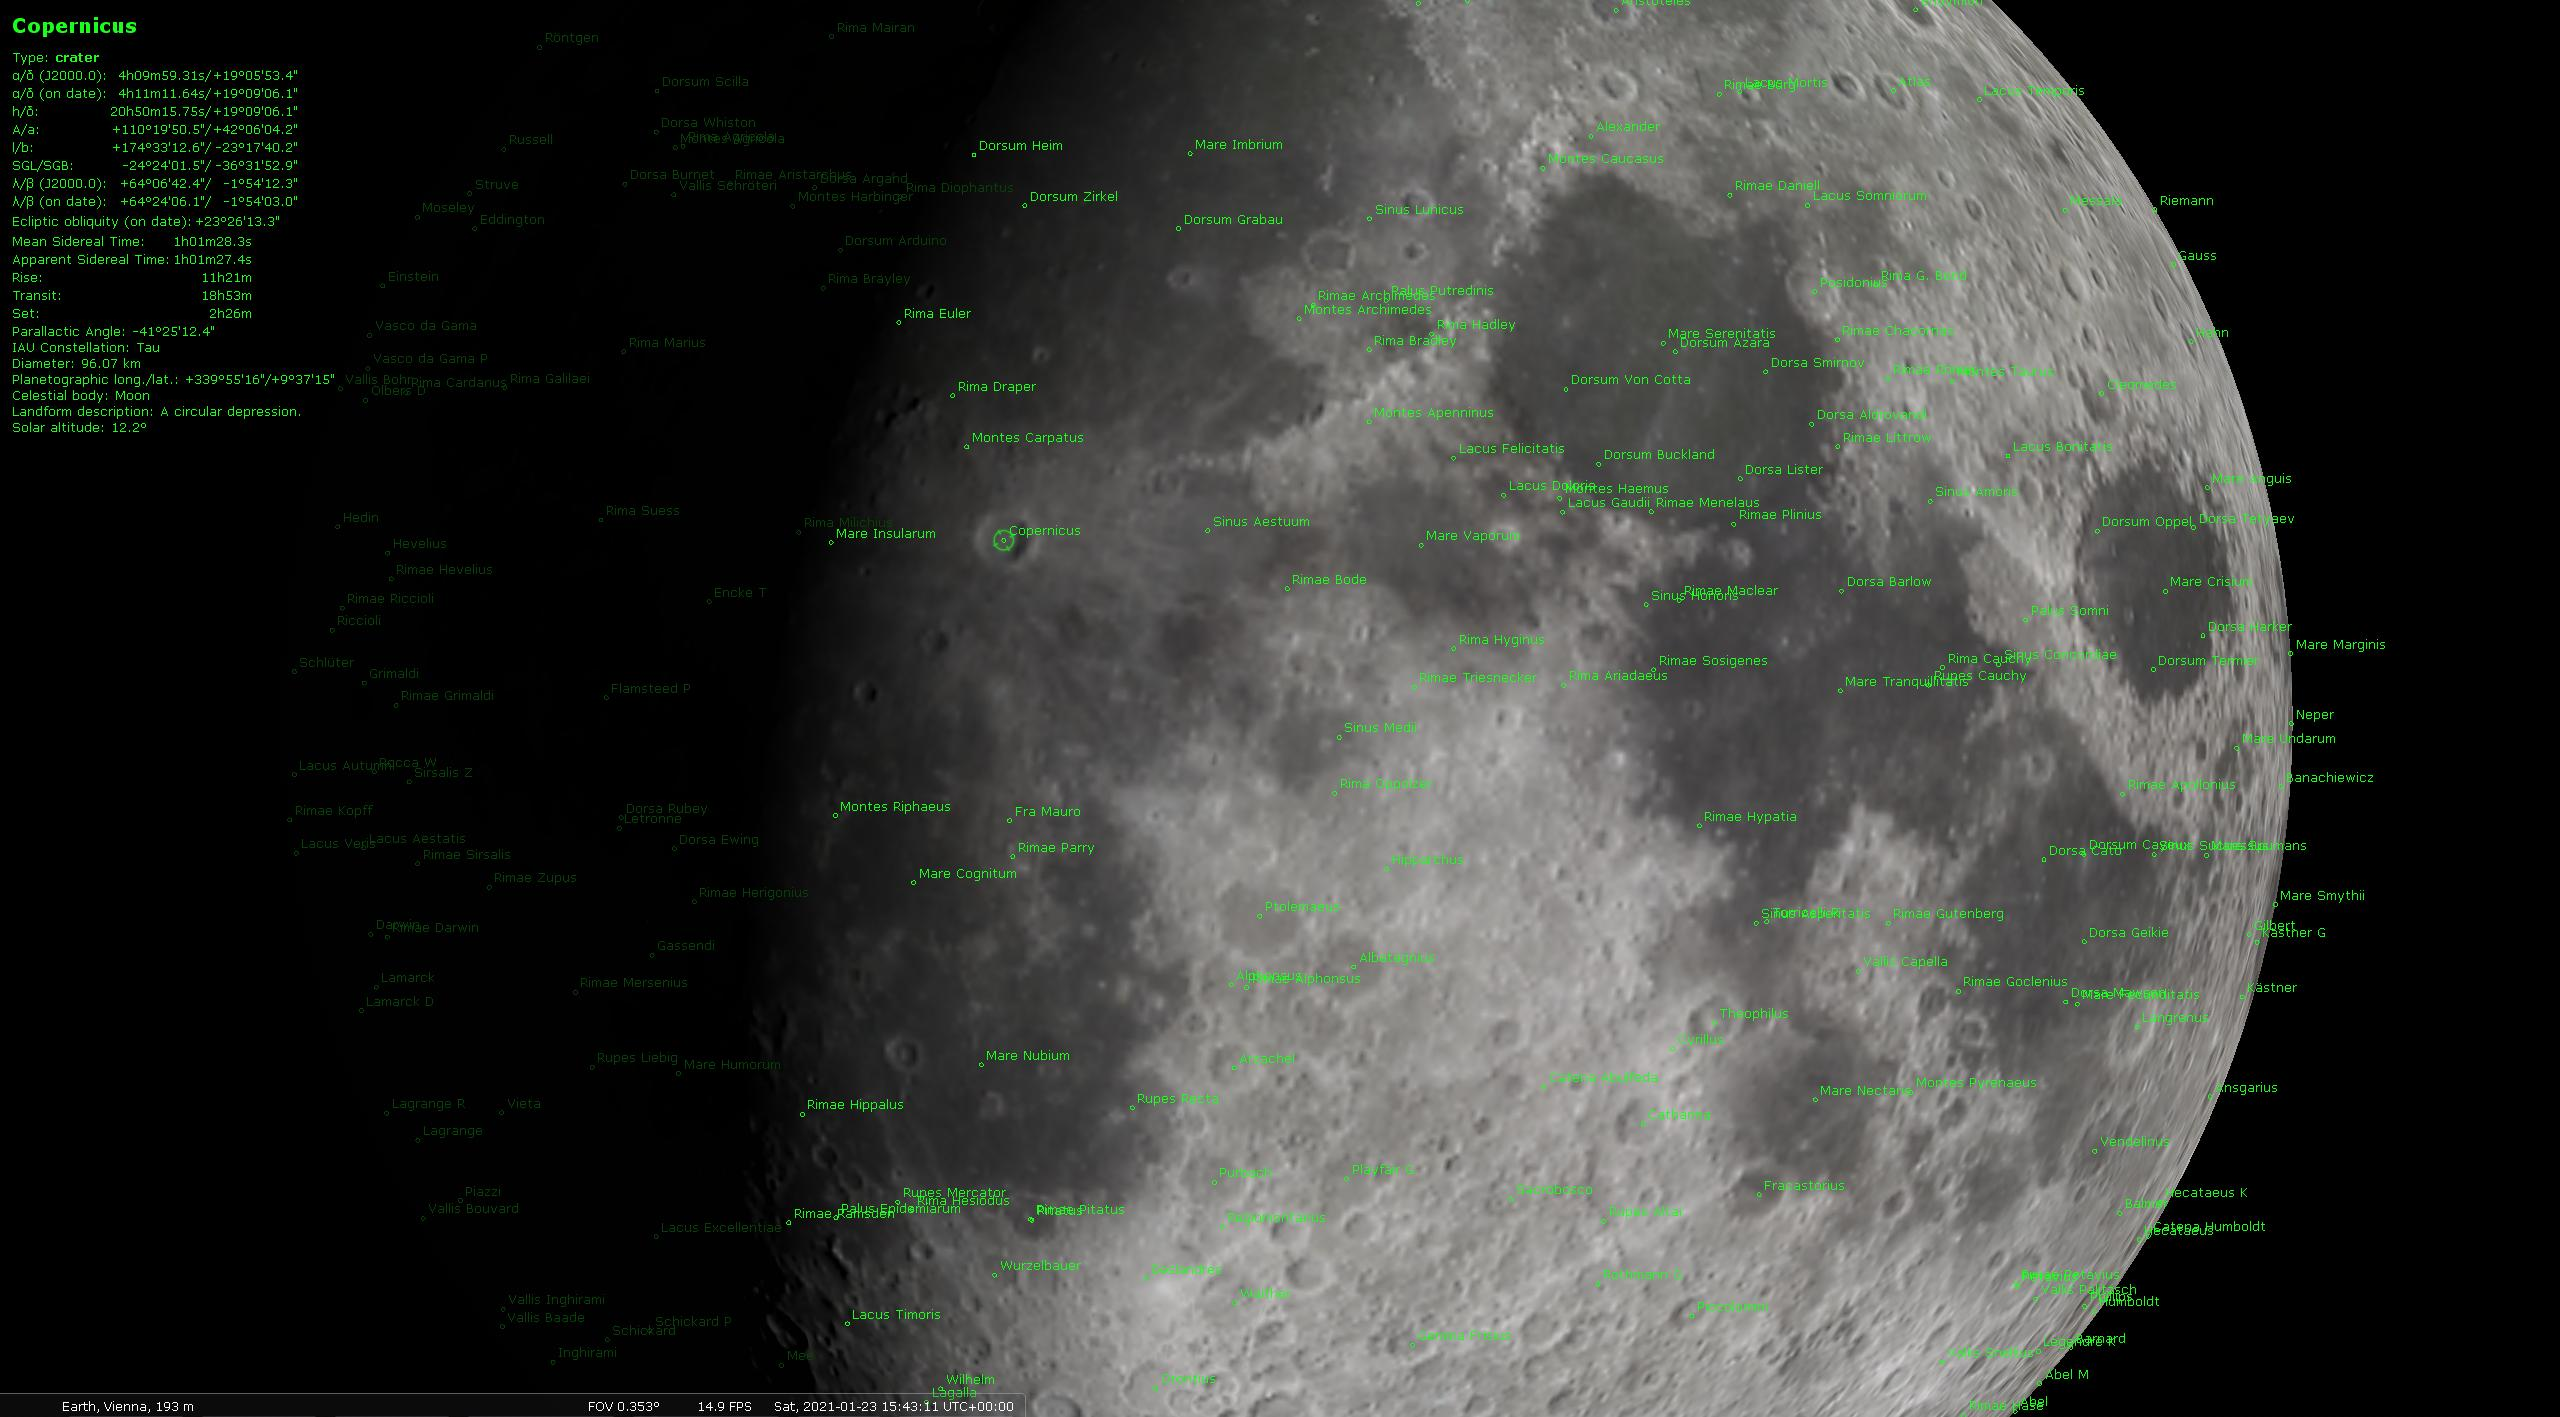
\includegraphics[width=\textwidth]{stellarium-nomenclature.jpg}
\caption{Feature nomenclature of the Moon.}
\label{fig:Nomenclature:Moon}
\end{figure}

Since version 0.17.0 Stellarium supports planetary nomenclature, which allows using the 
planetarium for educational and informative purposes on the one hand, and as tool for 
recognition and targeting of the planetary features for advanced amateurs on the other 
hand, avoiding the need for additional cartographic software in the field. 

All planetary nomenclature items are stored in a dedicated internal format, 
and all names are translatable to provide better understanding of those names 
by average users and newbies -- for example in schools or universities.  
Of course all nomenclature items are available for finding in the Search Tool 
after enabling the display of nomenclature (this feature is rather costly in terms of 
computing power and therefore is by default disabled in the GUI).

\emph{The information in sections \ref{sec:Nomenclature:ApprovingNames}--\ref{sec:Nomenclature:DescriptorTerms}, 
included here for reference, has been taken from the ``Gazetteer of Planetary Nomenclature'' website 
by the International Astronomical Union (IAU)\index{IAU} Working Group for Planetary System Nomenclature 
(WGPSN)}\footnote{\url{https://planetarynames.wr.usgs.gov}, visited on 2017-10-30}.

\section{Format of nomenclature data file}
\label{sec:Nomenclature:format}

File \file{data/nomenclature.fab} is a plain text file in UTF-8 encoding and has a very simple data format: 
\begin{itemize}
\item One item per line;
\item Each item contains seven elements with white space (``space'' or ``tab'' character) as delimiter.
\end{itemize}
File \file{data/nomenclature.dat} is a zipped \file{data/nomenclature.fab} file and used to minimize time of loading the data and reduce size of the installation package.

\begin{center}
\begin{tabularx}{\textwidth}{l|l|X}\toprule
\emph{Item}                              & \emph{Type} & \emph{Comment}\\\midrule
planet name                              & string  & English name of the planet, moon or minor body carrying the named feature\\%\midrule
ID of planetary feature                  & integer & unique integer, equal to Feature ID obtained from Gazetteer of Planetary Nomenclature\\%\midrule
translatable name of planetary feature   & string  & English name, containing context data for translators\\%\midrule
type of planetary feature                & string  & 2-char code (see \emph{designation} column in table in section \ref{sec:Nomenclature:DescriptorTerms})\\%\midrule
center latitude of planetary feature     & float   & decimal degrees\\%\midrule
center longitude of planetary feature    & float   & decimal degrees\\%\midrule
size of planetary feature                & float   & kilometers\\\bottomrule
\end{tabularx}
\end{center}

\noindent Example:
\begin{configfile}
Vesta 15201 _("Caesonia","crater") AA 31.20117 249.93457 104.23
\end{configfile}

\section{How names are approved by the IAU}
\label{sec:Nomenclature:ApprovingNames}\index{IAU}
When images are first obtained of the surface of a planet or satellite, a theme for naming features is chosen 
and a few important features are named, usually by members of the appropriate IAU task group (a commonly 
accepted planet-naming group). Later, as higher resolution images and maps become available, additional 
features are named at the request of investigators mapping or describing specific surfaces, features, 
or geologic formations. Anyone may suggest that a specific name be considered by a task group. 
If the members of the task group agree that the name is appropriate, it can be retained for use 
when there is a request from a member of the scientific community that a specific feature be named. 
Names successfully reviewed by a task group are submitted to the IAU Working Group for Planetary System 
Nomenclature (WGPSN)\footnote{Working Group for Planetary System Nomenclature -- \url{https://planetarynames.wr.usgs.gov/}}. 
Upon successful review by the members of the WGPSN, names are considered provisionally approved and can be 
used on maps and in publications as long as the provisional status is clearly stated. 
Provisional names are then presented for adoption to the IAU's General Assembly, which met triennially in the past, 
and which now adopts nomenclature for planetary surface features as required. A name is not considered to be 
official -- that is, ``adopted'' -- until the General Assembly has given its approval.

\section{IAU rules and conventions}
\label{sec:Nomenclature:RulesAndConventions}\index{IAU}
Names adopted by the IAU must follow various rules and conventions established and amended through the years by the Union. These include:
\begin{enumerate}
\item Nomenclature is a tool and the first consideration should be to make it simple, clear, and unambiguous.
\item In general, official names will not be given to features whose longest dimensions are less than 100 meters, 
      although exceptions may be made for smaller features having exceptional scientific interest.
\item The number of names chosen for each body should be kept to a minimum. Features should be 
      named only when they have special scientific interest, and when the naming of such features is useful 
	  to the scientific and cartographic communities at large.
\item Duplication of the same surface feature name on two or more bodies, and of the same name for satellites 
      and minor planets, is discouraged. Duplications may be allowed when names are especially appropriate and 
	  the chances for confusion are very small.
\item Individual names chosen for each body should be expressed in the language of origin. 
      Transliteration for various alphabets should be given, but there will be no translation from one language to another.
\item Where possible, the themes established in early solar system nomenclature should be used and expanded on.
\item Solar system nomenclature should be international in its choice of names. 
      Recommendations submitted to the IAU national committees will be considered, but final selection of the names 
	  is the responsibility of the International Astronomical Union. 
	  Where appropriate, the WGPSN strongly supports an equitable selection of names from ethnic groups, 
	  countries, and gender on each map; however, a higher percentage of names from the country planning a 
	  landing is allowed on landing site maps.
\item No names having political, military or religious significance may be used, except for names of political figures prior to the 19th century.
\item Commemoration of persons on planetary bodies should not normally be a goal in itself, 
      but may be employed in special circumstances and is reserved for persons of high and enduring international standing. 
	  Persons being so honored must have been deceased for at least three years, before a proposal may be submitted.
\item When more than one spelling of a name is extant, the spelling preferred by the person, or used in an authoritative reference, should be used. 
      Diacritical marks are a necessary part of a name and will be used.
\item Ring and ring-gap nomenclature and names for newly discovered satellites are developed in joint deliberation 
      between WGPSN and IAU Commission X2. Names will not be assigned to satellites until their orbital elements are 
	  reasonably well known or definite features have been identified on them.
\item Accessible and authoritative sources, including Internet sources, are required for adopted names. 
      Wikipedia is not sufficient as a source, but may be useful for identifying appropriate sources.
\end{enumerate}

\noindent In addition to these general rules, each task group develops additional conventions as it formulates an interesting 
and meaningful nomenclature for individual planetary bodies. Most of these conventions are self evident from study of the appendixes that follow.

\section{Naming conventions}
\label{sec:Nomenclature:NamingConventions}\index{IAU}
Names for all planetary features include a descriptor term, with a few exceptions. For craters, the descriptor term is implicit. 
Some features named on Io and Triton do not carry a descriptor term because they are ephemeral.

In general, the naming convention for a feature type remains the same regardless of its size. 
Exceptions to this rule are channels (valles) on Mars and Venus, and craters on the Moon, Mars, and Venus; 
naming conventions for these features differ according to size. 
The categories for naming features on each planet or satellite (and the exceptions) are listed in 
Categories for Naming Features on Planets and Satellites\footnote{%
   Surface Feature Categories -- \url{https://planetarynames.wr.usgs.gov/Page/Categories}}. 
One feature classification, regio, was originally used on early maps of the Moon and Mercury (drawn from telescopic observations) 
to describe vague albedo features. It is now also used to delineate a broad geographic region.

Named features on bodies so small that coordinates have not yet been determined are identified on drawings or images 
of the body that are included in the IAU Transactions volume of the year when the names were adopted. 
Satellite rings and gaps in the rings are named for scientists who have studied these features; 
drawings that show these names are also included in the pertinent Transactions volume. 
Names for atmospheric features are informal at present; a formal system will be chosen in the future.

The boundaries of many large features (such as terrae, regiones, planitiae, and plana) are not topographically or geomorphically distinct; 
the coordinates of these features are identified from an arbitrarily chosen center point. 
Boundaries (and thus coordinates) may be determined more accurately from geochemical and geophysical data obtained by future missions.

During active missions, small surface features are often given informal names. 
These may include landing sites, spacecraft impact sites, and small topographic features, such as craters, hills, and rocks. 
Such names will not be given official status by the IAU, except as provided for by Rule 2 above. 
As for the larger objects, official names for any such small features would have to conform to established IAU rules and categories.

When a satellite has been discovered through the efforts of a large scientific team, 
the list of individual team members may be too long to include all contributors. 
In such cases, credit for the discovery will go to the science team.

\newpage
\section{Descriptor terms (feature types)}
\label{sec:Nomenclature:DescriptorTerms}
Descriptor terms are intended to represent morphological characteristics, not geological origin. 
The WGPSN does not endorse any specific scientific hypotheses when assigning descriptors.

\begin{longtable}{l|c|p{72mm}}\toprule
\emph{Feature}        & \emph{Designation} & \emph{Description}\\\midrule
Albedo Feature        & AL & Geographic area distinguished by amount of reflected light\\%\midrule
Arcus, arcūs          & AR & Arc-shaped feature\\%\midrule
Astrum, astra         & AS & Radial-patterned features on Venus \\\midrule
Catena, catenae       & CA & Chain of craters \\%\midrule
Cavus, cavi           & CB & Hollows, irregular steep-sided depressions usually in arrays or clusters\\%\midrule
Chaos, chaoses        & CH & Distinctive area of broken terrain\\%\midrule
Chasma, chasmata      & CM & A deep, elongated, steep-sided depression\\%\midrule
Collis, colles        & CO & Small hills or knobs\\%\midrule
Corona, coronae       & CR & Ovoid-shaped feature\\%\midrule   
Crater, craters       & AA & A circular depression\\\midrule
Dorsum, dorsa         & DO & Ridge\\\midrule
Eruptive center       & ER & Active volcanic centers on Io\\\midrule
Facula, faculae       & FA & Bright spot\\%\midrule
Farrum, farra         & FR & Pancake-like structure, or a row of such structures\\%\midrule
Flexus, flexūs        & FE & A very low curvilinear ridge with a scalloped pattern\\%\midrule   
Fluctus, fluctūs      & FL & Flow terrain\\%\midrule
Flumen, flumina       & FM & Channel on Titan that might carry liquid\\%\midrule
Fossa, fossae         & FO & Long, narrow depression\\%\midrule
Fretum, freta         & FT & Strait, a narrow passage of liquid connecting two larger areas of liquid\\\midrule
Insula, insulae       & IN & Island (islands), an isolated land area (or group of such areas) surrounded by, 
                             or nearly surrounded by, a liquid area (sea or lake)\\\midrule
Labes, labēs          & LA & Landslide\\%\midrule   
Labyrinthus, labyrinthi & LB & Complex of intersecting valleys or ridges\\%\midrule
Lacuna, lacunae       & LU & Irregularly shaped depression on Titan having the appearance of a dry lake bed\\%\midrule
Lacus, lacūs          & LC & ``Lake'' or small plain; on Titan, a ``lake'' or small, 
                             dark plain with discrete, sharp boundaries\\%\midrule
Landing site name     & LF & Lunar features at or near Apollo landing sites\\%\midrule
Large ringed feature  & LG & Cryptic ringed features\\%\midrule
Lenticula, lenticulae & LE & Small dark spots on Europa\\%\midrule   
Linea, lineae         & LI & A dark or bright elongate marking, may be curved or straight\\%\midrule
Lingula, lingulae     & LN & Extension of plateau having rounded lobate or tongue-like boundaries\\\midrule
Macula, maculae       & MA & Dark spot, may be irregular\\%\midrule
Mare, maria           & ME & ``Sea''; on the Moon, low albedo, relatively smooth plain, generally of large extent; 
                             on Mars, dark albedo areas of no known geological significance; 
                             on Titan, large expanses of dark materials thought to be liquid hydrocarbons\\%\midrule
Mensa, mensae         & MN & A flat-topped prominence with cliff-like edges\\%\midrule
Mons, montes          & MO & Mountain\\\midrule   
Oceanus, oceani       & OC & A very large dark area on the moon\\\midrule
Palus, paludes        & PA & ``Swamp''; small plain\\%\midrule
Patera, paterae       & PE & An irregular crater, or a complex one with scalloped edges\\%\midrule
Planitia, planitiae   & PL & Low plain\\%\midrule
Planum, plana         & PM & Plateau or high plain\\%\midrule
Plume, plumes         & PU & Cryo-volcanic features on Triton\\%\midrule   
Promontorium, promontoria & PR & ``Cape''; headland promontoria\\\midrule
Regio, regiones       & RE & A large area marked by reflectivity or color distinctions from adjacent areas, 
                             or a broad geographic region\\%\midrule
Reticulum, reticula   & RT & Reticular (netlike) pattern on Venus\\%\midrule
Rima, rimae           & RI & Fissure\\%\midrule
Rupes, rupēs          & RU & Scarp\\\midrule
Satellite Feature     & SF & A feature that shares the name of an associated feature. 
                             For example, on the Moon the craters referred to as ``Lettered Craters'' 
							 are classified in the gazetteer as ``Satellite Features''\\%\midrule   
Saxum, saxa           & SA & Boulder or rock\\%\midrule
Scopulus, scopuli     & SC & Lobate or irregular scarp\\%\midrule
Serpens, serpentes    & SE & Sinuous feature with segments of positive and negative relief along its length\\%\midrule
Sinus, sinūs          & SI & ``Bay''; small plain; on Titan, bays within seas or lakes of liquid hydrocarbons\\%\midrule
Sulcus, sulci         & SU & Subparallel furrows and ridges\\\midrule
Terra, terrae         & TA & Extensive land mass\\%\midrule
Tessera, tesserae     & TE & Tile-like, polygonal terrain\\%\midrule   
Tholus, tholi         & TH & Small domical mountain or hill\\\midrule
Unda, undae           & UN & Dunes\\\midrule
Vallis, valles        & VA & Valley\\%\midrule
Vastitas, vastitates  & VS & Extensive plain\\%\midrule
Virga, virgae         & VI & A streak or stripe of color\\\bottomrule
\end{longtable}


\section*{Author and Acknowledgement}
\label{sec:Nomenclature:Acknowledgments}
The nomenclature feature has been implemented by Teresa Huertas Roldán supported by the ``ESA Summer of Code in Space 2017'' programme.

%%% Local Variables: 
%%% mode: latex
%%% TeX-master: "guide"
%%% End: 

